\documentclass{article} % For LaTeX2e
\usepackage{geometry}
\usepackage{graphicx}
\usepackage{booktabs}

\geometry{
  paperheight=11in,
  paperwidth=8.5in,
  top=0.5in,         % Top margin
  bottom=1in,         % Bottom margin
  left=0.75in,        % Left margin
  right=0.75in        % Right margin
}


% Optional math commands from https://github.com/goodfeli/dlbook_notation.
%%%%% NEW MATH DEFINITIONS %%%%%

\usepackage{amsmath,amsfonts,bm}

% Mark sections of captions for referring to divisions of figures
\newcommand{\figleft}{{\em (Left)}}
\newcommand{\figcenter}{{\em (Center)}}
\newcommand{\figright}{{\em (Right)}}
\newcommand{\figtop}{{\em (Top)}}
\newcommand{\figbottom}{{\em (Bottom)}}
\newcommand{\captiona}{{\em (a)}}
\newcommand{\captionb}{{\em (b)}}
\newcommand{\captionc}{{\em (c)}}
\newcommand{\captiond}{{\em (d)}}

% Highlight a newly defined term
\newcommand{\newterm}[1]{{\bf #1}}


% Figure reference, lower-case.
\def\figref#1{figure~\ref{#1}}
% Figure reference, capital. For start of sentence
\def\Figref#1{Figure~\ref{#1}}
\def\twofigref#1#2{figures \ref{#1} and \ref{#2}}
\def\quadfigref#1#2#3#4{figures \ref{#1}, \ref{#2}, \ref{#3} and \ref{#4}}
% Section reference, lower-case.
\def\secref#1{section~\ref{#1}}
% Section reference, capital.
\def\Secref#1{Section~\ref{#1}}
% Reference to two sections.
\def\twosecrefs#1#2{sections \ref{#1} and \ref{#2}}
% Reference to three sections.
\def\secrefs#1#2#3{sections \ref{#1}, \ref{#2} and \ref{#3}}
% Reference to an equation, lower-case.
\def\eqref#1{equation~\ref{#1}}
% Reference to an equation, upper case
\def\Eqref#1{Equation~\ref{#1}}
% A raw reference to an equation---avoid using if possible
\def\plaineqref#1{\ref{#1}}
% Reference to a chapter, lower-case.
\def\chapref#1{chapter~\ref{#1}}
% Reference to an equation, upper case.
\def\Chapref#1{Chapter~\ref{#1}}
% Reference to a range of chapters
\def\rangechapref#1#2{chapters\ref{#1}--\ref{#2}}
% Reference to an algorithm, lower-case.
\def\algref#1{algorithm~\ref{#1}}
% Reference to an algorithm, upper case.
\def\Algref#1{Algorithm~\ref{#1}}
\def\twoalgref#1#2{algorithms \ref{#1} and \ref{#2}}
\def\Twoalgref#1#2{Algorithms \ref{#1} and \ref{#2}}
% Reference to a part, lower case
\def\partref#1{part~\ref{#1}}
% Reference to a part, upper case
\def\Partref#1{Part~\ref{#1}}
\def\twopartref#1#2{parts \ref{#1} and \ref{#2}}

\def\ceil#1{\lceil #1 \rceil}
\def\floor#1{\lfloor #1 \rfloor}
\def\1{\bm{1}}
\newcommand{\train}{\mathcal{D}}
\newcommand{\valid}{\mathcal{D_{\mathrm{valid}}}}
\newcommand{\test}{\mathcal{D_{\mathrm{test}}}}

\def\eps{{\epsilon}}


% Random variables
\def\reta{{\textnormal{$\eta$}}}
\def\ra{{\textnormal{a}}}
\def\rb{{\textnormal{b}}}
\def\rc{{\textnormal{c}}}
\def\rd{{\textnormal{d}}}
\def\re{{\textnormal{e}}}
\def\rf{{\textnormal{f}}}
\def\rg{{\textnormal{g}}}
\def\rh{{\textnormal{h}}}
\def\ri{{\textnormal{i}}}
\def\rj{{\textnormal{j}}}
\def\rk{{\textnormal{k}}}
\def\rl{{\textnormal{l}}}
% rm is already a command, just don't name any random variables m
\def\rn{{\textnormal{n}}}
\def\ro{{\textnormal{o}}}
\def\rp{{\textnormal{p}}}
\def\rq{{\textnormal{q}}}
\def\rr{{\textnormal{r}}}
\def\rs{{\textnormal{s}}}
\def\rt{{\textnormal{t}}}
\def\ru{{\textnormal{u}}}
\def\rv{{\textnormal{v}}}
\def\rw{{\textnormal{w}}}
\def\rx{{\textnormal{x}}}
\def\ry{{\textnormal{y}}}
\def\rz{{\textnormal{z}}}

% Random vectors
\def\rvepsilon{{\mathbf{\epsilon}}}
\def\rvtheta{{\mathbf{\theta}}}
\def\rva{{\mathbf{a}}}
\def\rvb{{\mathbf{b}}}
\def\rvc{{\mathbf{c}}}
\def\rvd{{\mathbf{d}}}
\def\rve{{\mathbf{e}}}
\def\rvf{{\mathbf{f}}}
\def\rvg{{\mathbf{g}}}
\def\rvh{{\mathbf{h}}}
\def\rvu{{\mathbf{i}}}
\def\rvj{{\mathbf{j}}}
\def\rvk{{\mathbf{k}}}
\def\rvl{{\mathbf{l}}}
\def\rvm{{\mathbf{m}}}
\def\rvn{{\mathbf{n}}}
\def\rvo{{\mathbf{o}}}
\def\rvp{{\mathbf{p}}}
\def\rvq{{\mathbf{q}}}
\def\rvr{{\mathbf{r}}}
\def\rvs{{\mathbf{s}}}
\def\rvt{{\mathbf{t}}}
\def\rvu{{\mathbf{u}}}
\def\rvv{{\mathbf{v}}}
\def\rvw{{\mathbf{w}}}
\def\rvx{{\mathbf{x}}}
\def\rvy{{\mathbf{y}}}
\def\rvz{{\mathbf{z}}}

% Elements of random vectors
\def\erva{{\textnormal{a}}}
\def\ervb{{\textnormal{b}}}
\def\ervc{{\textnormal{c}}}
\def\ervd{{\textnormal{d}}}
\def\erve{{\textnormal{e}}}
\def\ervf{{\textnormal{f}}}
\def\ervg{{\textnormal{g}}}
\def\ervh{{\textnormal{h}}}
\def\ervi{{\textnormal{i}}}
\def\ervj{{\textnormal{j}}}
\def\ervk{{\textnormal{k}}}
\def\ervl{{\textnormal{l}}}
\def\ervm{{\textnormal{m}}}
\def\ervn{{\textnormal{n}}}
\def\ervo{{\textnormal{o}}}
\def\ervp{{\textnormal{p}}}
\def\ervq{{\textnormal{q}}}
\def\ervr{{\textnormal{r}}}
\def\ervs{{\textnormal{s}}}
\def\ervt{{\textnormal{t}}}
\def\ervu{{\textnormal{u}}}
\def\ervv{{\textnormal{v}}}
\def\ervw{{\textnormal{w}}}
\def\ervx{{\textnormal{x}}}
\def\ervy{{\textnormal{y}}}
\def\ervz{{\textnormal{z}}}

% Random matrices
\def\rmA{{\mathbf{A}}}
\def\rmB{{\mathbf{B}}}
\def\rmC{{\mathbf{C}}}
\def\rmD{{\mathbf{D}}}
\def\rmE{{\mathbf{E}}}
\def\rmF{{\mathbf{F}}}
\def\rmG{{\mathbf{G}}}
\def\rmH{{\mathbf{H}}}
\def\rmI{{\mathbf{I}}}
\def\rmJ{{\mathbf{J}}}
\def\rmK{{\mathbf{K}}}
\def\rmL{{\mathbf{L}}}
\def\rmM{{\mathbf{M}}}
\def\rmN{{\mathbf{N}}}
\def\rmO{{\mathbf{O}}}
\def\rmP{{\mathbf{P}}}
\def\rmQ{{\mathbf{Q}}}
\def\rmR{{\mathbf{R}}}
\def\rmS{{\mathbf{S}}}
\def\rmT{{\mathbf{T}}}
\def\rmU{{\mathbf{U}}}
\def\rmV{{\mathbf{V}}}
\def\rmW{{\mathbf{W}}}
\def\rmX{{\mathbf{X}}}
\def\rmY{{\mathbf{Y}}}
\def\rmZ{{\mathbf{Z}}}

% Elements of random matrices
\def\ermA{{\textnormal{A}}}
\def\ermB{{\textnormal{B}}}
\def\ermC{{\textnormal{C}}}
\def\ermD{{\textnormal{D}}}
\def\ermE{{\textnormal{E}}}
\def\ermF{{\textnormal{F}}}
\def\ermG{{\textnormal{G}}}
\def\ermH{{\textnormal{H}}}
\def\ermI{{\textnormal{I}}}
\def\ermJ{{\textnormal{J}}}
\def\ermK{{\textnormal{K}}}
\def\ermL{{\textnormal{L}}}
\def\ermM{{\textnormal{M}}}
\def\ermN{{\textnormal{N}}}
\def\ermO{{\textnormal{O}}}
\def\ermP{{\textnormal{P}}}
\def\ermQ{{\textnormal{Q}}}
\def\ermR{{\textnormal{R}}}
\def\ermS{{\textnormal{S}}}
\def\ermT{{\textnormal{T}}}
\def\ermU{{\textnormal{U}}}
\def\ermV{{\textnormal{V}}}
\def\ermW{{\textnormal{W}}}
\def\ermX{{\textnormal{X}}}
\def\ermY{{\textnormal{Y}}}
\def\ermZ{{\textnormal{Z}}}

% Vectors
\def\vzero{{\bm{0}}}
\def\vone{{\bm{1}}}
\def\vmu{{\bm{\mu}}}
\def\vtheta{{\bm{\theta}}}
\def\va{{\bm{a}}}
\def\vb{{\bm{b}}}
\def\vc{{\bm{c}}}
\def\vd{{\bm{d}}}
\def\ve{{\bm{e}}}
\def\vf{{\bm{f}}}
\def\vg{{\bm{g}}}
\def\vh{{\bm{h}}}
\def\vi{{\bm{i}}}
\def\vj{{\bm{j}}}
\def\vk{{\bm{k}}}
\def\vl{{\bm{l}}}
\def\vm{{\bm{m}}}
\def\vn{{\bm{n}}}
\def\vo{{\bm{o}}}
\def\vp{{\bm{p}}}
\def\vq{{\bm{q}}}
\def\vr{{\bm{r}}}
\def\vs{{\bm{s}}}
\def\vt{{\bm{t}}}
\def\vu{{\bm{u}}}
\def\vv{{\bm{v}}}
\def\vw{{\bm{w}}}
\def\vx{{\bm{x}}}
\def\vy{{\bm{y}}}
\def\vz{{\bm{z}}}

% Elements of vectors
\def\evalpha{{\alpha}}
\def\evbeta{{\beta}}
\def\evepsilon{{\epsilon}}
\def\evlambda{{\lambda}}
\def\evomega{{\omega}}
\def\evmu{{\mu}}
\def\evpsi{{\psi}}
\def\evsigma{{\sigma}}
\def\evtheta{{\theta}}
\def\eva{{a}}
\def\evb{{b}}
\def\evc{{c}}
\def\evd{{d}}
\def\eve{{e}}
\def\evf{{f}}
\def\evg{{g}}
\def\evh{{h}}
\def\evi{{i}}
\def\evj{{j}}
\def\evk{{k}}
\def\evl{{l}}
\def\evm{{m}}
\def\evn{{n}}
\def\evo{{o}}
\def\evp{{p}}
\def\evq{{q}}
\def\evr{{r}}
\def\evs{{s}}
\def\evt{{t}}
\def\evu{{u}}
\def\evv{{v}}
\def\evw{{w}}
\def\evx{{x}}
\def\evy{{y}}
\def\evz{{z}}

% Matrix
\def\mA{{\bm{A}}}
\def\mB{{\bm{B}}}
\def\mC{{\bm{C}}}
\def\mD{{\bm{D}}}
\def\mE{{\bm{E}}}
\def\mF{{\bm{F}}}
\def\mG{{\bm{G}}}
\def\mH{{\bm{H}}}
\def\mI{{\bm{I}}}
\def\mJ{{\bm{J}}}
\def\mK{{\bm{K}}}
\def\mL{{\bm{L}}}
\def\mM{{\bm{M}}}
\def\mN{{\bm{N}}}
\def\mO{{\bm{O}}}
\def\mP{{\bm{P}}}
\def\mQ{{\bm{Q}}}
\def\mR{{\bm{R}}}
\def\mS{{\bm{S}}}
\def\mT{{\bm{T}}}
\def\mU{{\bm{U}}}
\def\mV{{\bm{V}}}
\def\mW{{\bm{W}}}
\def\mX{{\bm{X}}}
\def\mY{{\bm{Y}}}
\def\mZ{{\bm{Z}}}
\def\mBeta{{\bm{\beta}}}
\def\mPhi{{\bm{\Phi}}}
\def\mLambda{{\bm{\Lambda}}}
\def\mSigma{{\bm{\Sigma}}}

% Tensor
\DeclareMathAlphabet{\mathsfit}{\encodingdefault}{\sfdefault}{m}{sl}
\SetMathAlphabet{\mathsfit}{bold}{\encodingdefault}{\sfdefault}{bx}{n}
\newcommand{\tens}[1]{\bm{\mathsfit{#1}}}
\def\tA{{\tens{A}}}
\def\tB{{\tens{B}}}
\def\tC{{\tens{C}}}
\def\tD{{\tens{D}}}
\def\tE{{\tens{E}}}
\def\tF{{\tens{F}}}
\def\tG{{\tens{G}}}
\def\tH{{\tens{H}}}
\def\tI{{\tens{I}}}
\def\tJ{{\tens{J}}}
\def\tK{{\tens{K}}}
\def\tL{{\tens{L}}}
\def\tM{{\tens{M}}}
\def\tN{{\tens{N}}}
\def\tO{{\tens{O}}}
\def\tP{{\tens{P}}}
\def\tQ{{\tens{Q}}}
\def\tR{{\tens{R}}}
\def\tS{{\tens{S}}}
\def\tT{{\tens{T}}}
\def\tU{{\tens{U}}}
\def\tV{{\tens{V}}}
\def\tW{{\tens{W}}}
\def\tX{{\tens{X}}}
\def\tY{{\tens{Y}}}
\def\tZ{{\tens{Z}}}


% Graph
\def\gA{{\mathcal{A}}}
\def\gB{{\mathcal{B}}}
\def\gC{{\mathcal{C}}}
\def\gD{{\mathcal{D}}}
\def\gE{{\mathcal{E}}}
\def\gF{{\mathcal{F}}}
\def\gG{{\mathcal{G}}}
\def\gH{{\mathcal{H}}}
\def\gI{{\mathcal{I}}}
\def\gJ{{\mathcal{J}}}
\def\gK{{\mathcal{K}}}
\def\gL{{\mathcal{L}}}
\def\gM{{\mathcal{M}}}
\def\gN{{\mathcal{N}}}
\def\gO{{\mathcal{O}}}
\def\gP{{\mathcal{P}}}
\def\gQ{{\mathcal{Q}}}
\def\gR{{\mathcal{R}}}
\def\gS{{\mathcal{S}}}
\def\gT{{\mathcal{T}}}
\def\gU{{\mathcal{U}}}
\def\gV{{\mathcal{V}}}
\def\gW{{\mathcal{W}}}
\def\gX{{\mathcal{X}}}
\def\gY{{\mathcal{Y}}}
\def\gZ{{\mathcal{Z}}}

% Sets
\def\sA{{\mathbb{A}}}
\def\sB{{\mathbb{B}}}
\def\sC{{\mathbb{C}}}
\def\sD{{\mathbb{D}}}
% Don't use a set called E, because this would be the same as our symbol
% for expectation.
\def\sF{{\mathbb{F}}}
\def\sG{{\mathbb{G}}}
\def\sH{{\mathbb{H}}}
\def\sI{{\mathbb{I}}}
\def\sJ{{\mathbb{J}}}
\def\sK{{\mathbb{K}}}
\def\sL{{\mathbb{L}}}
\def\sM{{\mathbb{M}}}
\def\sN{{\mathbb{N}}}
\def\sO{{\mathbb{O}}}
\def\sP{{\mathbb{P}}}
\def\sQ{{\mathbb{Q}}}
\def\sR{{\mathbb{R}}}
\def\sS{{\mathbb{S}}}
\def\sT{{\mathbb{T}}}
\def\sU{{\mathbb{U}}}
\def\sV{{\mathbb{V}}}
\def\sW{{\mathbb{W}}}
\def\sX{{\mathbb{X}}}
\def\sY{{\mathbb{Y}}}
\def\sZ{{\mathbb{Z}}}

% Entries of a matrix
\def\emLambda{{\Lambda}}
\def\emA{{A}}
\def\emB{{B}}
\def\emC{{C}}
\def\emD{{D}}
\def\emE{{E}}
\def\emF{{F}}
\def\emG{{G}}
\def\emH{{H}}
\def\emI{{I}}
\def\emJ{{J}}
\def\emK{{K}}
\def\emL{{L}}
\def\emM{{M}}
\def\emN{{N}}
\def\emO{{O}}
\def\emP{{P}}
\def\emQ{{Q}}
\def\emR{{R}}
\def\emS{{S}}
\def\emT{{T}}
\def\emU{{U}}
\def\emV{{V}}
\def\emW{{W}}
\def\emX{{X}}
\def\emY{{Y}}
\def\emZ{{Z}}
\def\emSigma{{\Sigma}}

% entries of a tensor
% Same font as tensor, without \bm wrapper
\newcommand{\etens}[1]{\mathsfit{#1}}
\def\etLambda{{\etens{\Lambda}}}
\def\etA{{\etens{A}}}
\def\etB{{\etens{B}}}
\def\etC{{\etens{C}}}
\def\etD{{\etens{D}}}
\def\etE{{\etens{E}}}
\def\etF{{\etens{F}}}
\def\etG{{\etens{G}}}
\def\etH{{\etens{H}}}
\def\etI{{\etens{I}}}
\def\etJ{{\etens{J}}}
\def\etK{{\etens{K}}}
\def\etL{{\etens{L}}}
\def\etM{{\etens{M}}}
\def\etN{{\etens{N}}}
\def\etO{{\etens{O}}}
\def\etP{{\etens{P}}}
\def\etQ{{\etens{Q}}}
\def\etR{{\etens{R}}}
\def\etS{{\etens{S}}}
\def\etT{{\etens{T}}}
\def\etU{{\etens{U}}}
\def\etV{{\etens{V}}}
\def\etW{{\etens{W}}}
\def\etX{{\etens{X}}}
\def\etY{{\etens{Y}}}
\def\etZ{{\etens{Z}}}

% The true underlying data generating distribution
\newcommand{\pdata}{p_{\rm{data}}}
% The empirical distribution defined by the training set
\newcommand{\ptrain}{\hat{p}_{\rm{data}}}
\newcommand{\Ptrain}{\hat{P}_{\rm{data}}}
% The model distribution
\newcommand{\pmodel}{p_{\rm{model}}}
\newcommand{\Pmodel}{P_{\rm{model}}}
\newcommand{\ptildemodel}{\tilde{p}_{\rm{model}}}
% Stochastic autoencoder distributions
\newcommand{\pencode}{p_{\rm{encoder}}}
\newcommand{\pdecode}{p_{\rm{decoder}}}
\newcommand{\precons}{p_{\rm{reconstruct}}}

\newcommand{\laplace}{\mathrm{Laplace}} % Laplace distribution

\newcommand{\E}{\mathbb{E}}
\newcommand{\Ls}{\mathcal{L}}
\newcommand{\R}{\mathbb{R}}
\newcommand{\emp}{\tilde{p}}
\newcommand{\lr}{\alpha}
\newcommand{\reg}{\lambda}
\newcommand{\rect}{\mathrm{rectifier}}
\newcommand{\softmax}{\mathrm{softmax}}
\newcommand{\sigmoid}{\sigma}
\newcommand{\softplus}{\zeta}
\newcommand{\KL}{D_{\mathrm{KL}}}
\newcommand{\Var}{\mathrm{Var}}
\newcommand{\standarderror}{\mathrm{SE}}
\newcommand{\Cov}{\mathrm{Cov}}
% Wolfram Mathworld says $L^2$ is for function spaces and $\ell^2$ is for vectors
% But then they seem to use $L^2$ for vectors throughout the site, and so does
% wikipedia.
\newcommand{\normlzero}{L^0}
\newcommand{\normlone}{L^1}
\newcommand{\normltwo}{L^2}
\newcommand{\normlp}{L^p}
\newcommand{\normmax}{L^\infty}

\newcommand{\parents}{Pa} % See usage in notation.tex. Chosen to match Daphne's book.

\DeclareMathOperator*{\argmax}{arg\,max}
\DeclareMathOperator*{\argmin}{arg\,min}

\DeclareMathOperator{\sign}{sign}
\DeclareMathOperator{\Tr}{Tr}
\let\ab\allowbreak


\usepackage{hyperref}
\usepackage{url}
\usepackage{natbib}
\usepackage{float}
\usepackage[font=small,labelfont=bf,margin=0.5in]{caption}

% Make every table slightly smaller (text inside tables uses \small)
\usepackage{etoolbox}
\AtBeginEnvironment{table}{\small}


\title{Something in the Way: Deep Learning for Crater Detection and Crater-Aware Route Planning on Mars}

\author{Enes Demirel\\
\texttt{mdemire1@depaul.edu} 
}
\date{\today}

\begin{document}


\maketitle

\begin{abstract}
It takes approximately 4 to 22 minutes for a signal to reach Mars; therefore, Mars rovers are increasingly driven autonomously. To do this, it is important for these rovers to be able to recognize dangers such as craters without help from Earth. In this project, we study two questions: (1) which type of deep learning model performs best at detecting craters in orbital images of Mars, and (2) whether the model's mistakes matter for rovers. Using about 52,000 labeled satellite images, we compare three models: a U-Net trained from scratch, a Faster R-CNN fine-tuned from a model trained on everyday objects, and a frozen DINOv3 foundation model with only a small layer trained on top. We find that Faster R-CNN performs best with an $F_1$ score of 0.80, while U-Net achieves 0.57 and DINOv3 0.21. We also show that it is important to use multiple scoring methods in crater detection, as pixel-based scores can make very different models appear equally good. We then use the best detector's map to drive two simulated rovers. Rover~1 plans its full route with A*, while Rover~2 is a small neural network that learns to drive from A*'s moves, only seeing the area around itself. Both reach their goals on all 1,000 test routes, but most of the crater entries come not from missed craters, but from detected craters with slightly wrong outlines.
\end{abstract}

\vspace{-10pt}
\section{Introduction}
\label{sec:introduction}
Mars is the most habitable planet in our solar system after Earth, so it is the next step in human exploration. However, because we are not yet able to send humans to Mars; we need to rely on rovers to do the work for us. A signal from Earth to Mars, or vice versa, takes 4 to 22 minutes to reach its destination, so engineers do not have the luxury of steering a rover in real time \cite{nasa_drive}. Instead, the rover has to drive itself and for a rover to drive on its own, it is very important to be able to identify dangers on its own.

One of the most common dangers on the Martian surface is craters. One catalog alone lists more than three hundred thousand craters, and it counts only those wider than 1~km \cite{robbins2012}. It is important for the rover to know where the craters are when planning a safe route, because if it ends up in one, it can get stuck or tip over, and there is no one to fix it. With the help of satellites, we do have orbital images that show the large areas of Mars at once, but there are far too many craters to mark by hand. This is why deep learning models are important for automatically detecting them.

However, building models to detect craters raises two questions. First, which kind of model works best? We can train a model from scratch on crater images, fine-tune a model already trained to find everyday objects \cite{lin2014}, or use a foundation model that has learned general image features without labels. Second, do the detector's mistakes actually matter for the rover? A missed crater can lead the rover straight into it, while a false crater only makes its path a little longer. Even a good model can still miss a crater on the rover's path and cause it to crash, failing the mission, while a model with a lower score might play it safe and get the rover to its goal.

In this project, we study both questions on a public dataset of about 52,000 orbital images of the Martian surface with labeled craters \cite{hsu2021}. First, we build crater detection networks in three different ways: a U-Net convolutional neural network (CNN) \cite{ronneberger2015} trained from scratch; a Faster R-CNN \cite{ren2015} fine-tuned from a model that already detects everyday objects; and a DINOv3 \cite{simeoni2025} foundation model that we keep frozen, adding only a small layer on top of it. Then, we use the best model to drive two simulated rovers. Rover~1 sees the full map of detected craters and plans its whole route in advance with A* \cite{hart1968}. Rover~2 is a small neural network that only sees the area around itself and learns by imitating A*’s moves. Finally, we compare how often each rover reaches its goal, how often it enters a crater, and whether those craters were the ones the detector missed.


\vspace{-10pt}
\section{Related Work}
\label{sec:related_work}

Crater detection is a special case of semantic segmentation, in which every pixel in the image gets a label \cite{long2015}. Silburt et al. trained a U-Net to find craters in elevation maps of the Moon, and it found 92\% of the labeled craters \cite{silburt2019}. DeLatte et al. applied a deeper U-Net to orbital images of Mars \cite{delatte2019}, and Chen et al. further improved it and trained it on THEMIS infrared images with labels from the Robbins catalog \cite{robbins2012}, the same sources our dataset is built from \cite{chen2023}. The success of U-Net in these papers motivated us to use a U-Net for the train-from-scratch model. However, all of these papers build a single model and judge it only with detection scores, without testing what its mistakes mean for a rover. We compare three different ways of building a model and test them on basic rover simulations.

For the rover, we follow a method that teaches a neural network to drive by copying an expert, called behavior cloning, which was first introduced with ALVINN, which learned to steer a vehicle from a human driver's actions \cite{pomerleau1989, pomerleau1991}. Our Rover~2 uses the same idea with A* as the expert.
\vspace{-10pt}
\section{Preliminary and Background}
\label{sec:background}


\paragraph{The crater detection problem.}
Each image $x$ in our dataset is a $256 \times 256$ grid of pixels. Its mask $y$ is a grid of the same size that marks every pixel as crater ($y_i = 1$) or not ($y_i = 0$). We use two different ways for a model to find objects in an image. A detection model, such as Faster R-CNN, draws boxes around objects, each box with a confidence score. A segmentation model, such as our U-Net, instead gives every pixel $i$ a probability score $p_i$ of being a crater. In both cases, whether a pixel or a box, we use the cutoff $\tau$ to determine what counts as a crater or not. A higher cutoff gives fewer but more confident detections.

Craters are among the most common features on the Martian surface. However, most craters are small, so even in heavily cratered images, most of the pixels belong to the surrounding terrain. This is called class imbalance, a well-known problem in machine learning in which one class vastly outnumbers the others. We see the same problem in our dataset, where only about 2\% of the pixels in a single image belong to craters.

\paragraph{How we judge the detectors.}
Intersection over union (IoU) measures how well a predicted area $A$ overlaps a true area $B$:
\begin{equation}
\text{IoU}(A, B) = \frac{|A \cap B|}{|A \cup B|},
\end{equation}
where 1 means a perfect match and 0 means no overlap. Pixel IoU compares a predicted mask to the true mask, but it counts pixels rather than craters. A model can still get a good score by finding only the large craters, which cover thousands of pixels, while missing the small ones. Therefore, we also want to know how many craters a model actually finds, and we score each crater separately.

A predicted crater counts as finding a real one if their boxes have an IoU of at least 0.5, and each real crater can be found only once. Counting the real craters that were found ($TP$), the predictions that matched no real crater ($FP$), and the real craters that were missed ($FN$), we compute
\begin{equation}
\text{P} = \frac{TP}{TP + FP}, \qquad
\text{R} = \frac{TP}{TP + FN}, \qquad
F_1 = \frac{2 \, \text{P} \, \text{R}}{\text{P} + \text{R}}.
\end{equation}
Precision (P) is the share of predictions that are real craters, and recall (R) is the share of real craters that were found. $F_1$ combines the two into one number, so a model cannot score well by marking everything as a crater (high recall, low precision) or by marking only the most obvious craters (high precision, low recall).

\paragraph{The rover simulation.}
Each rover navigates on a grid map, where every cell is either open or blocked by a crater. A rover moves from a start cell $s$ to a goal cell $g$ one step at a time. It can move into one of the 8 neighboring cells, with a cost of 1 for a straight move and $\sqrt{2}$ for a diagonal one.

Since the focus of this project is on the deep learning models, we keep the rover simulations simple and make a few assumptions. Our dataset only marks craters, so they are our only obstacles. All the maps are bird's-eye views derived from orbital imagery. The rover is modeled as a single point on the grid, where each cell corresponds to approximately 100~m on Mars. The rover always knows where it is, every move lands exactly where it was intended, and it can step in any of the eight directions without slipping or changing speed. Finally, we do not model the rover's physics or dynamics.

\vspace{-10pt}
\section{Methodology}
\label{sec:methodology}

\begin{figure}[t]
  \centering
  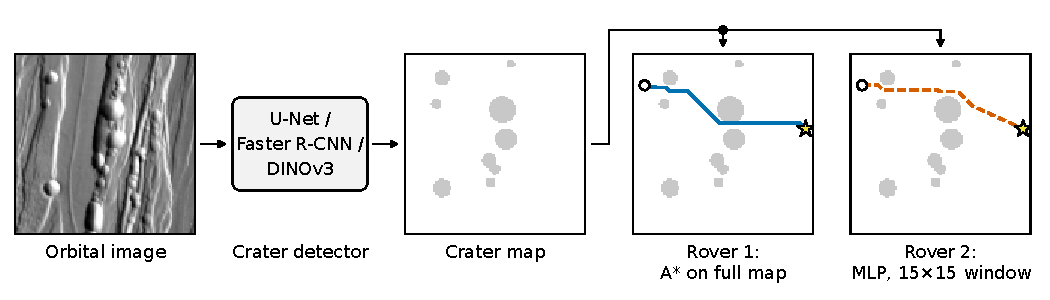
\includegraphics[width=0.8\textwidth]{figures/pipeline.pdf}
  \caption{Overview of our pipeline, where a crater detector turns an orbital satellite image into a map of craters. Rover~1 plans its full route on this map with A*, while Rover~2 is a small network that only sees a $15 \times 15$ window around itself. Both of them start at the white circle and drive to the star.}
  \label{fig:pipeline}
\end{figure}


\paragraph{Input Representation.}
Each training example is a single $256 \times 256$ grayscale image, where each pixel corresponds to approximately 0.1km on Mars. Each pixel value is scaled to the range 0 to 1. The labels are boxes around each crater, defined by their corner, width, and height. Faster R-CNN predicts boxes directly, so it uses the original boxes. However, for segmentation models, we convert each box into a filled circle centered at the same point and with a radius equal to half the box's longer side, and use these circles as a mask. Finally, both pretrained models were built for color images, so we copy the grayscale image into three identical channels. For DINOv3, we also normalize each channel with the same mean and standard deviation it was trained with.

\paragraph{Crater Detectors.}
In this project, we used three main approaches to build a model for identifying craters. A model trained from scratch starts with random weights and learns everything from our satellite images and labels. For this approach, we use U-Net \cite{ronneberger2015}, a neural network designed for pixel-level segmentation, and the same type of model that Silburt et al. used for lunar craters \cite{silburt2019}. A U-Net's encoder shrinks the image three times to capture the bigger picture, and its decoder then scales it back up to full size. However, because shrinking loses fine details in the image, skip connections are used to pass these details directly from the encoder to the decoder. It gives one score per pixel and has 1.9M parameters.

Fine-tuning is a form of transfer learning that starts with a model already trained on a different task, such as object detection. Later, it continues to train on our own data. Therefore, it does not need to relearn basic image features such as shapes and edges. Here, we use a Faster R-CNN \cite{ren2015} with a ResNet-50 \cite{he2016} backbone, trained on a large dataset of everyday objects. We replace its last layer so it predicts only two classes: crater or background. Normally, Faster R-CNN works by enlarging images to $800 \times 800$, but for the sake of training speed, our model keeps them at their original $256 \times 256$. In total, 41.1M of its parameters are trained.


Finally, to test whether a label-free model would perform well on finding craters on Mars, we use a foundation model, which is a very large model trained, usually, on millions or billions of images without labels. It learns general features of an image, such as edges, corners, and shapes, without being tied to a single task. Its weights are kept frozen, and only a small layer on top of it is trained. Here, we use the small version of DINOv3 \cite{simeoni2025}, which has 21.6M parameters. This model cuts each image into patches of $16 \times 16$ and describes each patch with 384 numbers. The small layer on top, which is called the head, is a $1 \times 1$ convolution (385 parameters in total) that maps each patch to a crater score. Later, these scores are stretched back to $256 \times 256$.

For the U-Net and DINOv3, each connected group of crater pixels becomes one predicted crater, so all three models can be scored in the same way.

\paragraph{Training.}
Because of the class imbalance problem described in Section~\ref{sec:background}, with the usual binary  cross-entropy loss, a model can achieve a small loss by predicting ``no crater'' almost everywhere. To prevent this, we use a weighted version of it that makes a mistake on a crater pixel cost more:


\begin{equation}
L = -\frac{1}{N} \sum_{i=1}^{N} \Big[ w \, y_i \log p_i + (1 - y_i) \log (1 - p_i) \Big],
\label{eq:weighted_bce}
\end{equation}
where $N$ is the number of pixels and $w$ is the penalty. We set $w = 10$ for the U-Net and the DINOv3 head. Faster R-CNN uses boxes to predict instead of pixels, so it keeps its own loss.  
Table~\ref{tab:training} lists the settings for each model.

\begin{table}[t]
  \centering
  \begin{tabular}{llllll}
    \toprule
    Model & Loss & Optimizer & Learning rate & Epochs & Batch size \\
    \midrule
    U-Net & Eq.~\ref{eq:weighted_bce} & Adam & $10^{-3}$, cosine & 15 & 16 \\
    Faster R-CNN & detection losses & SGD & $5 \times 10^{-3}$, cosine & 15 & 8 \\
    DINOv3 head & Eq.~\ref{eq:weighted_bce} & Adam & $10^{-3}$, cosine & 15 & 64 \\
    MLP, CNN (baselines) & Eq.~\ref{eq:weighted_bce} & Adam & $10^{-3}$, constant & 10 & 16 \\
    \bottomrule
  \end{tabular}
  \caption{Training settings for each model. Adam \cite{kingma2014} is the optimizer, and cosine is the cosine learning-rate schedule \cite{loshchilov2016}.}
  \label{tab:training}
\end{table}

To see how much the model design matters, we also trained two simpler baselines with the same loss: an MLP (multilayer perceptron) and a basic CNN (convolutional neural network) with eight convolutions and no downsampling, unlike U-Net.

All settings were chosen from a small number of options with giving most attention to defaults (details in appendix~\ref{sec:appendix}), and all detectors were trained on an NVIDIA RTX 5090 GPU. For each model, we keep the weights and the cutoff $\tau$ with the best validation score. All models except Faster R-CNN reached their best score before their final epoch, therefore they did not need any more training with higher amount of epochs. Faster R-CNN reached its best score at its final epoch, but its validation F1 stayed between the 0.79 and 0.80 over the last epochs, so more training would likely not improve. In addition, due to model size and time constraints, we chose not to train it any further.

\paragraph{Rovers.}
Rover~1 sees the whole map, while Rover~2 sees only a small $15 \times 15$ window of it. Both use the crater map generated by Faster R-CNN, our best detector, with a 0.8 cutoff. We use an algorithm called A* \cite{hart1968} to find the shortest path between $s$ and $g$ that avoids the craters. It explores the grid by always picking the cell with the lowest cost so far plus an estimate of the distance left to the goal. Rover 1 plans the entire route before moving.

Rover~2 learns to drive using behavior cloning, a method that teaches a neural network to make decisions by learning from an expert. It works like a classic classification problem. The data comes from A* planning on the true crater map, and the network is a small MLP with 8 outputs, one for each move the rover can take. The input is what the agent sees in a given moment, and the label is the action the expert took. After training with many examples, the network predicts an action for each new input. Therefore, Rover~2 works by predicting what A* would do in each step, using only its $15 \times 15$ window and the direction to the goal. A known limitation of this method is that the expert never makes mistakes, so the training data never shows how to recover from one. After a single wrong move, the network can end up in situations it has never seen.


\vspace{-10pt}
\section{Numerical Experiments}
\label{sec:numerical_experiments}

\paragraph{Setup.}
Our Mars crater dataset comes from the 2022 GeoAI Martian Challenge \cite{hsu2021} and consists of orbital images with crater labels from the Robbins catalog \cite{robbins2012}. The challenge's own test images have no labels, so we keep only the 51,838 labeled images and split them randomly using the 80/10/10 rule, resulting in 41,470 for training, 5,184 for validation, and 5,184 for testing. All models used the same split. We choose the best epoch and the cutoff on the validation set, and all reported numbers are on the test set.

We test both rovers on the same routes using 1,000 different test images, selecting the start and goal from random cells that are free in both the true and detected crater maps and are at least 150 cells apart. Rover~2 is trained on the training and validation data, so the test images are new to it. A trip counts as reaching the goal if the rover arrives at it, or, for Rover~2, if it gets within 2 cells of it. We also record each true crater where the rovers enter, and count it as missed by the detector if no detected box overlaps it with an IoU of at least 0.5. Path lengths are measured with the same rule mentioned in Section~\ref{sec:background}.

\begin{table}[tb]
  \centering
  \begin{tabular}{llrcccc}
    \toprule
    Model & Approach & Trained params & Precision & Recall & $F_1$ & Pixel IoU \\
    \midrule
    MLP & from scratch & 0.5M & 0.067 & 0.316 & 0.110 & 0.176 \\
    CNN & from scratch & 0.2M & 0.031 & 0.634 & 0.059 & 0.215 \\
    \midrule
    U-Net & from scratch & 1.9M & 0.481 & 0.703 & 0.571 & \textbf{0.511} \\
    Faster R-CNN & fine-tuned & 41.1M & \textbf{0.795} & \textbf{0.803} & \textbf{0.799} & -- \\
    DINOv3 & frozen + head & 385 & 0.306 & 0.158 & 0.209 & 0.508 \\
    \bottomrule
  \end{tabular}
  \caption{Crater detection results on the test set. Pixel IoU uses each model's pixel cutoff chosen on validation: 0.8 for U-Net and DINOv3, and 0.5 for the baselines (Faster R-CNN predicts boxes, so it has none). Per-crater scores use a 0.5 cutoff for the baselines and the best validation cutoff for the main models. \textbf{Bold} means best.}
  \label{tab:detectors}
\end{table}

\paragraph{Crater detection results.}

Table~\ref{tab:detectors} shows the results of all models on the test set. We can see that both of the baselines perform very poorly. Both of them are not capable of seeing a whole crater at once, and both reached a pixel IoU of only about 0.2.

When we move to the main detectors, we can see that U-Net, which can see a much larger area of the image, doubles the score. Therefore, we can conclude that the model's design clearly matters.

Among the main detectors, Faster R-CNN is clearly the winner. It has an $F_1$ score of 0.80, with very close precision and recall scores. Therefore, we can also say that it is the most balanced. The U-Net finds most of the craters with a recall of 0.70, but fewer than half of its detections are real, with a precision of 0.48, because its masks contain many small groups of pixels that are not craters. On the other hand, DINOv3 has the opposite problem. It misses most of the craters with a recall score of 0.16. The problem is likely that each of its $16 \times 16$ patches blends craters into the surrounding ground.

We can also see the benefit of using two different ways of measuring success in our models when we looked at DINOv3 and U-Net. This is because even though they have almost the same pixel IoU (0.511 and 0.508), which means the models are about equally good per pixel, U-Net's per-crater score is almost three times better ($F_1$ of 0.57 against 0.21). The baselines show the same effect as well; while CNN's IoU score is better, it scores lower per crater. Therefore, we conclude that pixel IoU alone can obscure how well a model actually finds a crater, and that having an additional way to score models and a balanced way to decide the winner is much more reliable.

\begin{table}[t]
  \centering
  \begin{tabular}{lcc}
    \toprule
    & Rover 1 (A*, full map) & Rover 2 (MLP, $15 \times 15$ window) \\
    \midrule
    Reached the goal & 100\% & 100\% \\
    Routes that entered a crater & 9.3\% & 11.2\% \\
    Craters entered & 100 & 117 \\
    \quad missed by the detector & 32 & 23 \\
    \bottomrule
  \end{tabular}
  \caption{Rover results on the same 1,000 test routes.}
  \label{tab:rovers}
\end{table}

\paragraph{Rover results.}
Table~\ref{tab:rovers} compares the two rovers on the same 1,000 test routes. We can see that both of them reach the goal on every route. Rover~1 enters a true crater in 9.3\% of its routes, 100 craters in total, where 32 of them were missed by the detector and the other 68 were detected, but their circles were slightly off, so the rover drove into their edges. This shows that the precision of circle size and placement when detecting craters is as important as detecting the craters themselves. Hence, to answer our second question, missed craters do matter, but most crater entries come from imprecise crater outlines rather than misses.

While Rover~2 also reaches the goal as often, even when seeing only a $15 \times 15$ window and predicting the best move at each step, it enters more craters (11.2\% of routes). Out of 117 craters it entered, only 23 were missed by the detector. This means that most were craters that Rover~2 could see but still drove into, which either happened because of the same outline mistake as discussed for Rover~1 or due to the downsides of behavior cloning discussed in Section~\ref{sec:methodology}. Three more example routes for each rover are shown in Appendix~\ref{sec:appendix}.








\vspace{-10pt}
\section{Conclusion}
\label{sec:conclusion}

We set out to determine whether deep learning could be useful for identifying craters on Mars's surface to help rovers plan their own routes. Our goal was to identify which kind of models detect craters the best, and whether a detector's mistakes matter for a rover. The fine-tuned Faster R-CNN performed the best ($F_1$ of 0.80), while U-Net trained from scratch produced many false alarms, and the frozen DINOv3 missed most craters. We also saw that having two different ways to score our models was useful, since two models with almost the same pixel IoU score did not necessarily find craters equally well. For the rovers, most crater entries came from detected craters with slightly wrong outlines, not from missed craters.

It is also important to note that our work here has some limitations. Instead of enlarging the image to $800 \times 800$ to capture finer details, we used $256 \times 256$ images to keep training fast for Faster R-CNN. DINOv3 was kept frozen, which likely hurt it on small craters. As mentioned above, our labels are boxes turned into circles; therefore, they only approximate the real crater shapes. In addition, many small craters were not labeled, some of which our detectors might have found but were counted as false detection, lowering their precision. The rover simulation is also simple, and Rover~2 only copies A*, so it never learns from its own mistakes.

Future work could include training the Faster R-CNN model on enlarged images, fine-tuning DINOv3, adding a small safety margin around detected craters, and training Rover~2 with a model that can learn from its own mistakes.





\clearpage
\bibliography{refs}
\bibliographystyle{plain}

\appendix
\vspace{-10pt}
\section{Appendix}
\label{sec:appendix}

\subsection{Training details}
\label{app:training}
This table shows how we trained each model.
\begin{table}[H]
  \centering
  \begin{tabular}{llllccl}
    \toprule
    Model & Optimizer & Learning rate & Schedule & Epochs & Batch & \\
    \midrule
    MLP & Adam & $10^{-3}$ & constant & 10 & 16  \\
    CNN & Adam & $10^{-3}$ & constant & 10 & 16  \\
    U-Net & Adam & $10^{-3}$ & cosine & 15 & 16  \\
    DINOv3 head & Adam & $10^{-3}$ & cosine & 15 & 64 \\
    Faster R-CNN & SGD (momentum 0.9, weight decay $5 \times 10^{-4}$) & $5 \times 10^{-3}$ & cosine & 15 & 8  \\
    Rover~2 MLP & Adam & $10^{-3}$ & constant & 10 & 256  \\
    \bottomrule
  \end{tabular}
  \caption{Full training settings. Adam uses its default settings and no weight decay.}
  \label{tab:app_training}
\end{table}

\clearpage
\subsection{Model selection}
\label{app:selection}
For each model, we kept the version that did best on the validation set. The first table shows which epoch and cutoffs we kept. The second table shows how the U-Net and DINOv3 scores change as the cutoff goes up.


\begin{table}[H]
  \centering
  \begin{tabular}{llccc}
    \toprule
    Model & Selected on & Best epoch & Pixel cutoff & Per-crater cutoff \\
    \midrule
    MLP & validation pixel IoU & 6 & 0.5 (fixed) & 0.5 (fixed) \\
    CNN & validation pixel IoU & 7 & 0.5 (fixed) & 0.5 (fixed) \\
    U-Net & validation pixel IoU & 10 & 0.8 & 0.9 \\
    DINOv3 & validation pixel IoU & 13 & 0.8 & 0.9 \\
    Faster R-CNN & validation $F_1$ & 15 & -- & 0.8 \\
    \bottomrule
  \end{tabular}
  \caption{Chosen epoch and cutoffs for each model. The pixel cutoff gives the best validation pixel IoU; the per-crater cutoff gives the best validation $F_1$ (Table~\ref{tab:app_cutoffs}). Faster R-CNN predicts boxes, so it has no pixel cutoff.}
  \label{tab:app_selection}
\end{table}

\begin{table}[H]
  \centering
  \begin{tabular}{ccc}
    \toprule
    Cutoff & U-Net & DINOv3 \\
    \midrule
    0.5 & 0.239 & 0.104 \\
    0.6 & 0.331 & 0.137 \\
    0.7 & 0.419 & 0.173 \\
    0.8 & 0.517 & 0.205 \\
    0.9 & \textbf{0.582} & \textbf{0.214} \\
    \bottomrule
  \end{tabular}
  \caption{Per-crater validation $F_1$ at each cutoff.}
  \label{tab:app_cutoffs}
\end{table}

\subsection{Validation and test results}
\label{app:valtest}
This table puts the validation and test scores side by side. MLP and CNN only have test scores.


\begin{table}[H]
  \centering
  \begin{tabular}{lcccccc}
    \toprule
    & \multicolumn{3}{c}{Validation} & \multicolumn{3}{c}{Test} \\
    \cmidrule(lr){2-4} \cmidrule(lr){5-7}
    Model & Precision & Recall & $F_1$ & Precision & Recall & $F_1$ \\
    \midrule
    MLP & -- & -- & -- & 0.067 & 0.316 & 0.110 \\
    CNN & -- & -- & -- & 0.031 & 0.634 & 0.059 \\
    U-Net & 0.498 & 0.700 & 0.582 & 0.481 & 0.703 & 0.571 \\
    DINOv3 & 0.311 & 0.163 & 0.214 & 0.306 & 0.158 & 0.209 \\
    Faster R-CNN & 0.793 & 0.797 & 0.795 & 0.795 & 0.803 & 0.799 \\
    \bottomrule
  \end{tabular}
  \caption{Per-crater scores on the validation and test sets.}
  \label{tab:app_valtest}
\end{table}

\clearpage
\subsection{Rover details}
\label{app:rovers}
This table lists how Rover~2 is built and trained, and the rules for its trips. The figure below shows some example routes from both rovers.

\begin{table}[H]
  \centering
  \begin{tabular}{ll}
    \toprule
    Item & Value \\
    \midrule
    Network & MLP, 227 $\to$ 128 (ReLU) $\to$ 8, 30,216 parameters \\
    Input & $15 \times 15$ window of the detected map + direction to the goal \\
    Labels & A* moves on the true crater map \\
    Training data & 88,252 examples from 500 training routes \\
    Validation data & 18,409 examples from 100 validation routes \\
    Validation accuracy & 75.3\% \\
    Reached the goal & within 2 cells of the goal \\
    Step limit & $3 \times$ the obstacle-free distance from start to goal \\
    Move off the map & the rover stays in place \\
    \bottomrule
  \end{tabular}
  \caption{Rover~2 details.}
  \label{tab:app_rover2}
\end{table}

\begin{figure}[H]
  \centering
  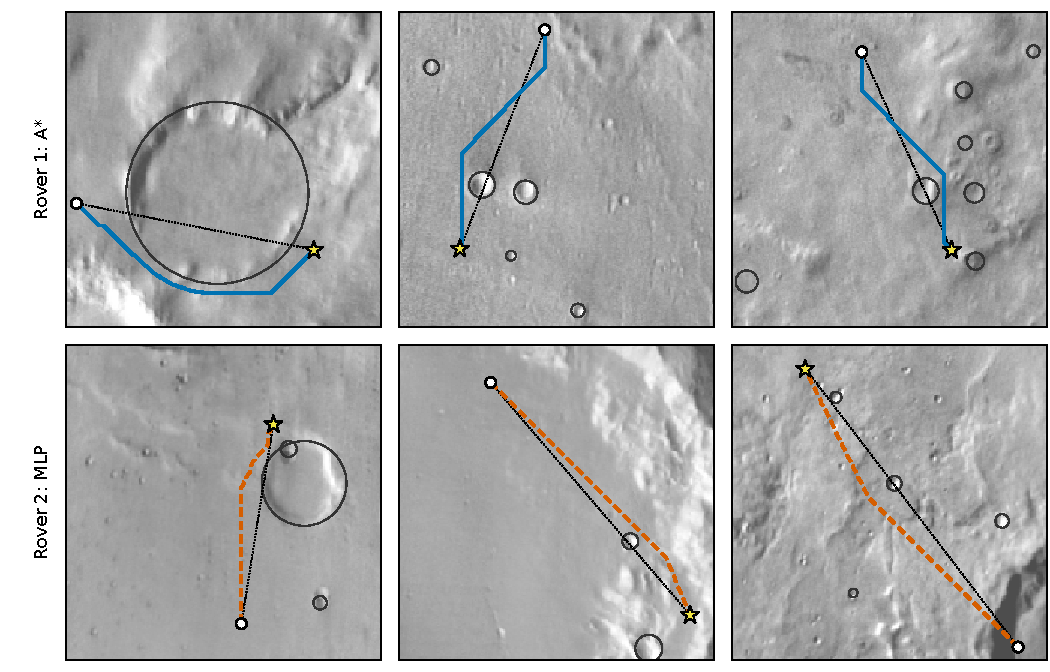
\includegraphics[width=\textwidth]{figures/rover_routes.pdf}
  \caption{Example routes. Top row: Rover~1. Bottom row: Rover~2. Both start at the white circle and drive to the star.}
  \label{fig:rover_routes}
\end{figure}

\end{document}